\documentclass[10pt,a4paper]{article}
\usepackage{algorithm}
\usepackage{algorithmicx}
\usepackage{algpseudocode}
\usepackage{amsfonts}
\usepackage{amsmath}
\usepackage{amssymb}
\usepackage{bbm}
\usepackage[a4paper, portrait, margin=1in]{geometry}
\usepackage{graphicx}
\usepackage[utf8]{inputenc}
\author{Nathan Cunningham}
\title{MDI SMC: Progress Report}
\begin{document}
\maketitle

\section*{Work completed}
\begin{algorithm}
\caption{Gibbs sampler}
 \begin{algorithmic}[1]
  \State Initialise $\Gamma$ matrix of prior allocation weights and $\Phi$ matrix of dataset concordance values
  \For{i = 1, \dots, number of iterations}
  \State Conditional on $\Gamma_{i-1}$ and $\Phi_{i-1}$ update the cluster labels, $c_{i}$, using alg. \ref{alg:pf}
  \State Conditional on $c_{i}$ update $\Gamma_i$ and $\Phi_i$
  \EndFor
\end{algorithmic}
\end{algorithm}


\begin{algorithm}
\caption{Particle filter to update cluster allocations}
\label{alg:pf}
 \begin{algorithmic}[1]
  \For{i = 1, \dots, n} \Comment{Loop over observations}
  \For{m = 1, \dots, M} \Comment{Loop over particles}
  \For{j = 1, \dots, d} \Comment{Loop over datasets}
  \State Sample $c^{(m)}_{i, j}$ \Comment{Propose a cluster for each datum}
  \State $q(c^{(m)}_{i,j} = k) \propto k^*(y_{i,j}|c_{i,j}^{(m)} = k) \gamma_{i, k, j}(1+\phi_{i})$
  \State $\xi^(m) =  \xi^(m) + \gamma_{i, k, j}(1+\phi_{i})k^*(y_{i,k}|c_{i,j}^{(m)} = k)$ 
  \EndFor
  \EndFor
  \EndFor

\end{algorithmic}
\end{algorithm}

Where
\begin{equation}
\label{eq:likelihood}
k^*(y_{i, k}|c_{i, k}^{(m)} = k) = (\mathbf{y_{i, k}} - \mathbf{\mu_k}) \mathbf{\Sigma^{-1}} (\mathbf{y_{i, k}} - \mathbf{\mu_k})^\top
\end{equation}
\begin{equation}
\label{eq:phi}
\Phi \text{ is a measure of cluster label correspondence across datasets}
\end{equation}
\begin{equation}
\label{eq:gamma}
\gamma_{i, k, j} \text{ is a prior weight for assigning observation i, in dataset k to cluster j}
\end{equation}

\noindent
Previously, it was suggested that eqn \ref{eq:likelihood} be calculated as the \texttt{logMarginalLikelihood} value output from the \texttt{Gaussian} function. However, this represents the likelihood of the cluster given the data point being assigned to it, as opposed to the likelihood of the data arising from a specific cluster. Using this as such resulted in all observations being assigned to a single cluster, or being allocated incorrectly to clusters.

\noindent
Using eqn \ref{eq:likelihood}
\begin{itemize}
\item Empty clusters are assumed to arise from a multivariate standard normal distribution, that with mean-vector $0$ and covariance matrix equal to the identity matrix. The data are normalised prior initially, so this is reasonable.
\item Non-empty clusters are assumed to have covariance matrix:
\begin{equation}
\frac{\mathbb{I}}{((n_{c,k,m}/a^(m)) + (1 / (1 - a^(m))) }
\end{equation}
where $n_{c,k,m}$ represents the number of observations in dataset k have been assigned to cluster c in particle m and $a^{(m)}$ is a measure of central tendency sampled for each particle from a beta distribution. This is based on the code in \cite{griffin2014sequential} and performs better than calculating a covariance from the observations already allocated to the cluster.
\end{itemize}

These problems become less prevalent as you progress through observations as clusters are more `settled'. This means that the clustering of data early in the dataset can be more uncertain. This can be seen in Fig. 1 where the data include two clusters, sorted within the dataset such that cluster 2 occurs subsequent to cluster 1.
Cluster 2 is well-discovered by the algorithm, as evidenced by the large dark grey square. Cluster 1 is much more poorly-defined. The tick marks are the suggested partition of the data into clusters (the algorithm is run here attempting to partition the data into 5 clusters).

This is in contrast to Fig. 2 where there is clear evidence of two distinct clusters. As the model is trying to partition the data into 5 subsets, the clusterings are more uncertain. Re-running the algorithm to search for two components gives greater certainty.

The dataset used for this is trivially simple to cluster, as shown in \ref{fig:testdata} the data are very distinctly separable. I also tested a more complicated dataset, shown in Fig. \ref{fig:gaussiandata}. The data were generated with five clusters. I ran the algorithm to search for a maximum of 10 clusters for relatively few iterations (100) and with relatively few particles (10), yet the data appears to successfully recover the true five clusters.

  


\begin{figure}[H]
\label{fig:noshuffle}
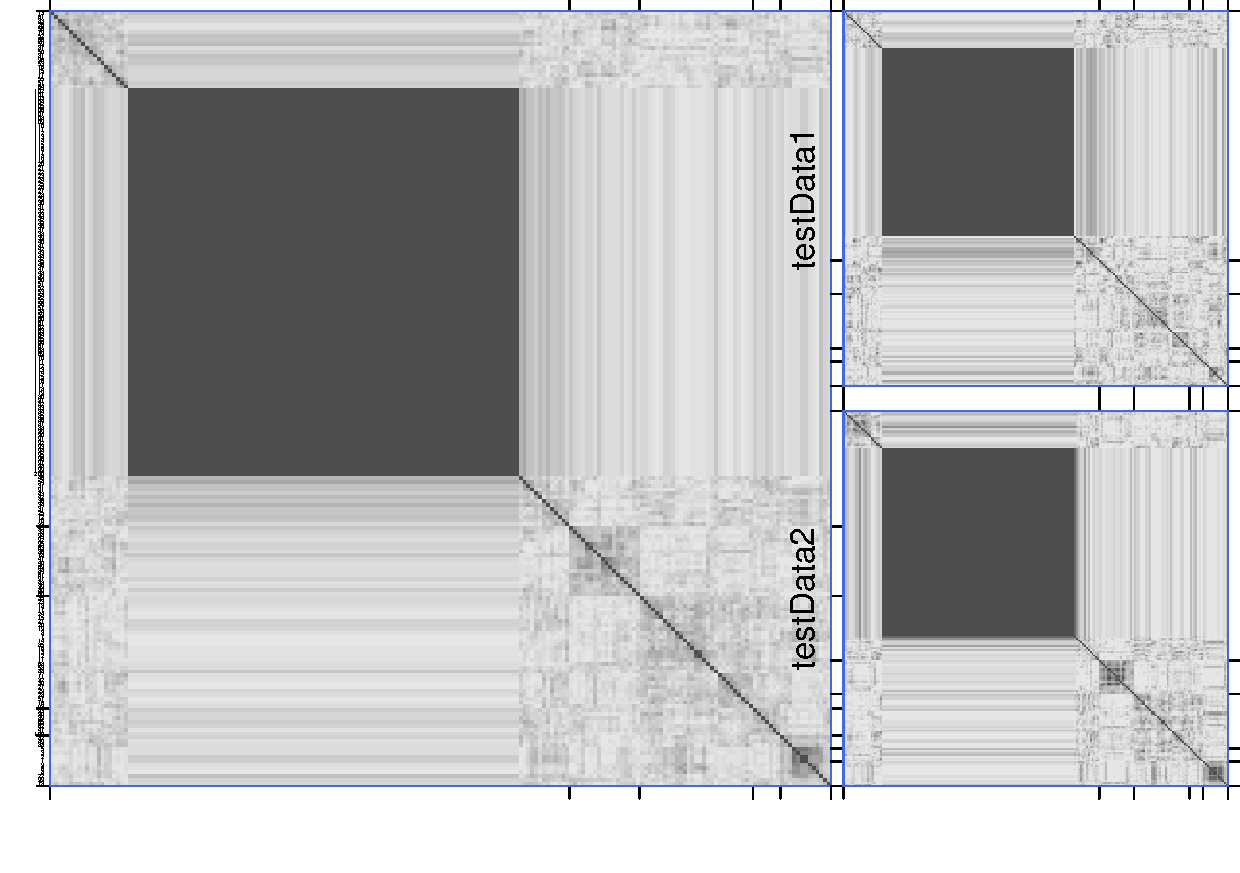
\includegraphics[width = \linewidth]{plots/noshuffle.pdf}
\caption{Cluster allocation agreement for mixture of Gaussian data with two clusters. Darker colours indicate greater agreement of allocations across runs of the algorithm. The smaller panels represent the posterior similarity matrix for each dataset, while the larger panel represents the consensus. The data are not shuffled prior to running the particle filter.}
\end{figure}

\begin{figure}[H]
\label{fig:shuffle}
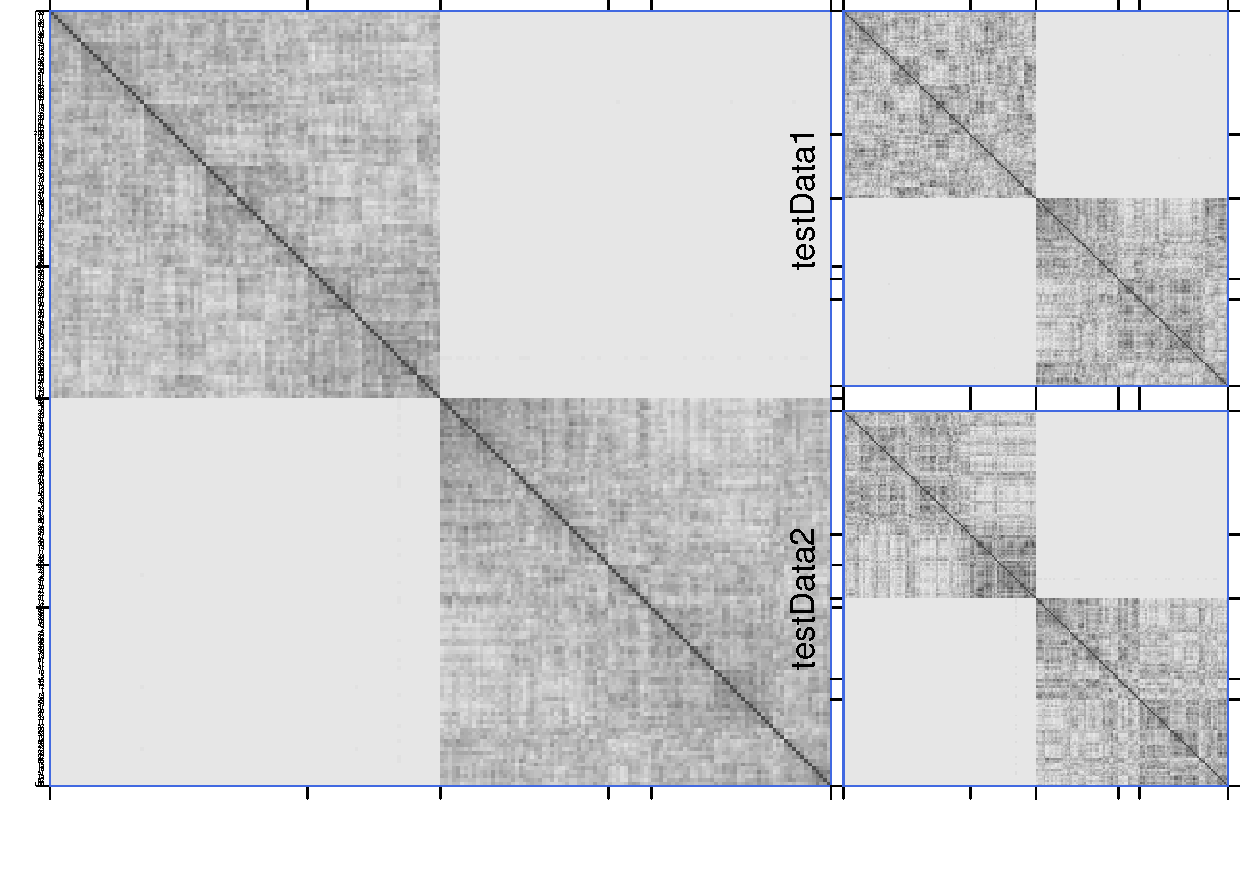
\includegraphics[width = \linewidth]{plots/shuffle.pdf}
\caption{Cluster allocation agreement for mixture of Gaussian data with two clusters. Darker colours indicate greater agreement of allocations across runs of the algorithm. The smaller panels represent the posterior similarity matrix for each dataset, while the larger panel represents the consensus. The data are shuffled prior to each run of the particle filter.}
\end{figure}

\begin{figure}[H]
\label{fig:testdata}
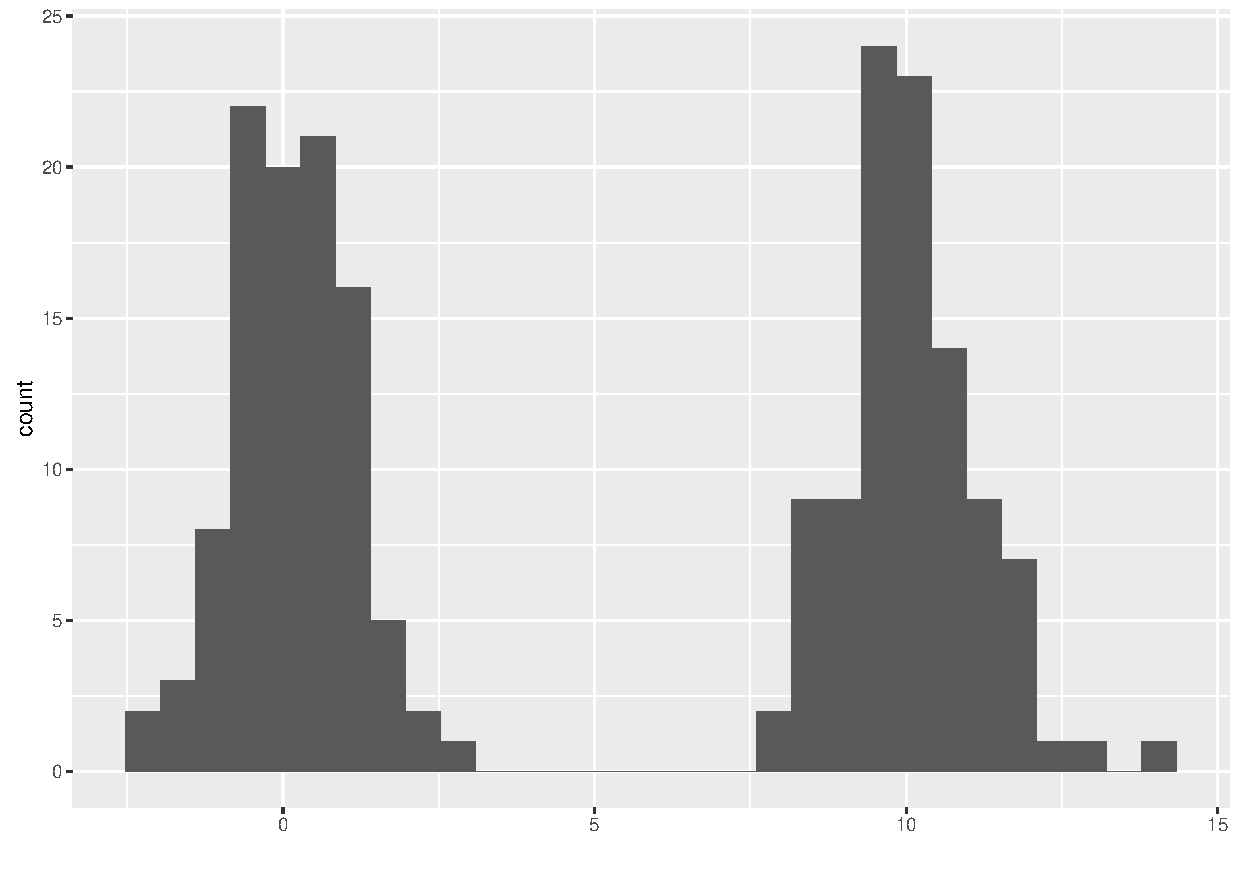
\includegraphics[width = \linewidth]{plots/testdata1_hist.pdf}
\caption{Synthetic data used for testing with two very distinct clusters defined by a gaussian distribution.}
\end{figure}

\begin{figure}[H]
\label{fig:gaussiandata}
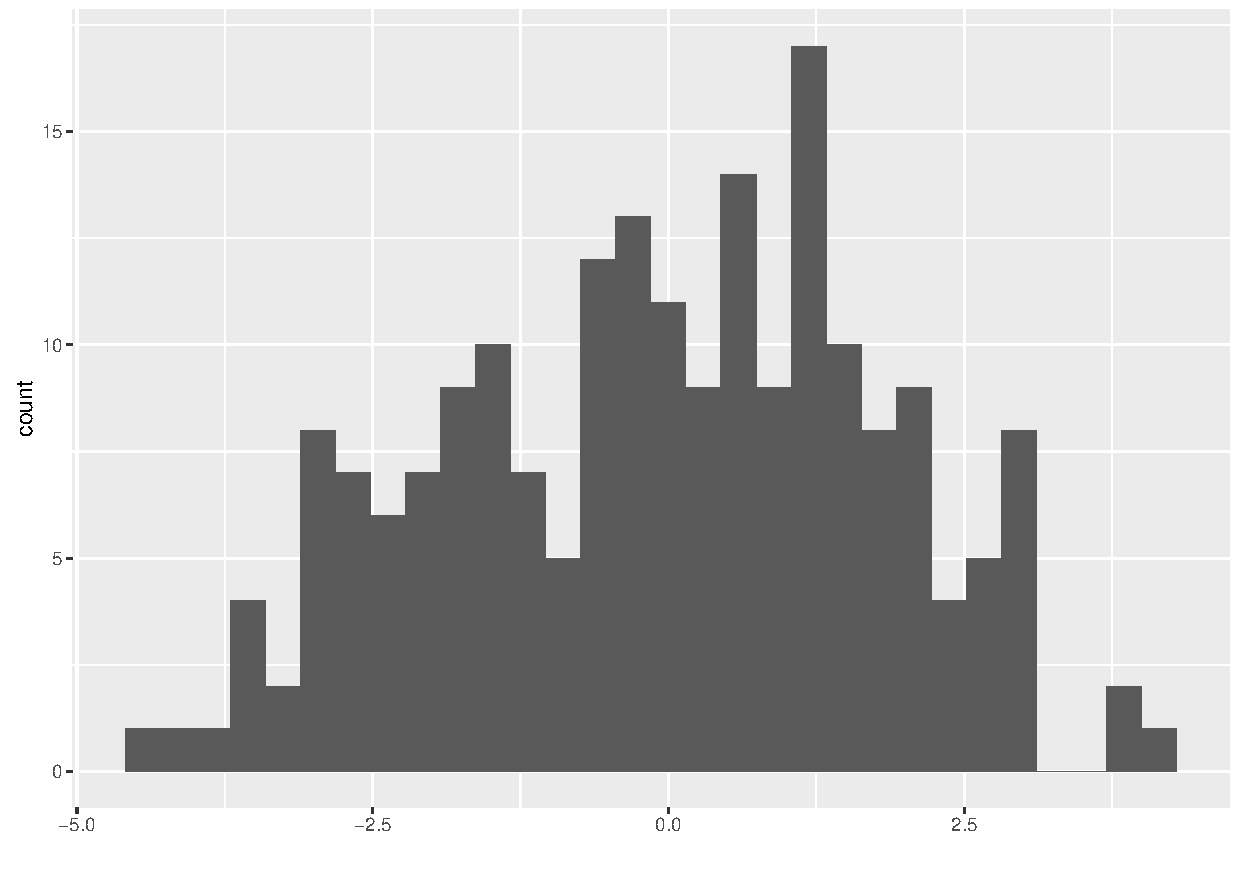
\includegraphics[width = \linewidth]{plots/gaussiandata1_hist.pdf}
\caption{Synthetic data used for testing with five non-distinct clusters each originating from a gaussian distribution.}
\end{figure}

\begin{figure}[H]
\label{fig:gaussiancluster}
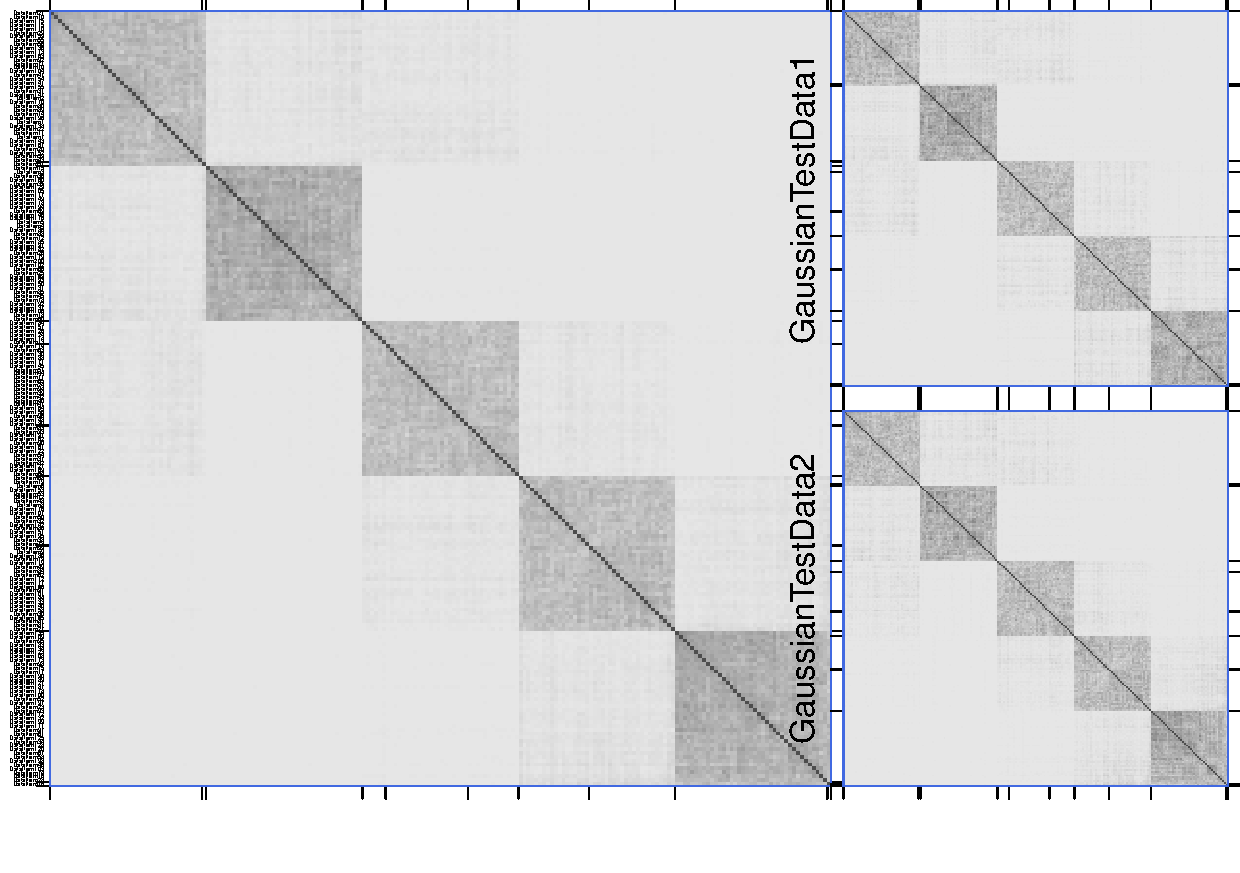
\includegraphics[width = \linewidth]{plots/gaussianclust.pdf}
\caption{Posterior similarity matrix for mixture of Gaussian data with five clusters. Darker colours indicate greater agreement of allocations across runs of the algorithm. The smaller panels represent the posterior similarity matrix for each dataset, while the larger panel represents the consensus. The algorithm is aiming to looking to partition the data into 10 clusters, however it appears to find the 5 true clusters.}
\end{figure}

\section*{Problems}
\begin{itemize}
\item Is the form of the covariance matrix an issue? It appears to run well within the dataset.
\item Is the shuffling of the data between runs an issue?
\item The algorithm currently is quite slow. Using 100 particles in the more complicated example above can result in a single iteration of the Gibbs sampler taking upwards of 30 seconds to run. Parallelisation may help here.
\item As the MDI algorithm originally was not set up for multiple particles, a single particle is selected at the end of the particle filter (based on $xi^(m)$) and that is fed into the next step of the Gibbs sampler. A possible solution would be to treat the particles as like separate datasets, so all the particles are returned and the $\Gamma$ and $\Phi$ values are updated based on all of the particles. Not sure if that's a good idea.
\end{itemize}



\bibliographystyle{plain}
\bibliography{bibliography.bib}

\end{document}